\documentclass{article}
\usepackage{graphicx} % Required for inserting images

\title{Group 5 Lab 2 Report}
\author{Ashley Björs,Elliot Bodin,Daniel Rytenberg,Jonas Gerne}
\date{January 2024}

\begin{document}
\maketitle

\section{Workflow}
Step 5 is dependent on step 4, which contains the previous steps(FaultInjector, ArithLogic, Max4bit8to1). This allowed for each step to be worked on seperatly and up until the simulation and test stages in step 4 and step 5. 
For step 4 and step 5 it was assumed that the previous entities worked correctly.
Working like this spread out the work load evenly amongst the group and if one completed their part they could help out the other group memebers, and lead to quickly being able to test and simulate. 

\section{LUT list}

\begin{figure}[h]
    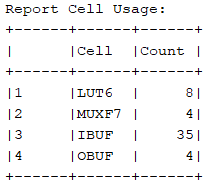
\includegraphics[width=5cm]{{Images/Lut 2.png}}
    \centering
    \caption{This is the LUT list of step 1}
\end{figure}

\begin{figure}[h]
    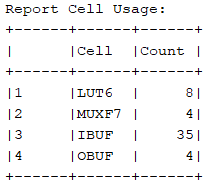
\includegraphics[width=5cm]{{Images/Lut 2.png}}
    \centering
    \caption{This is the LUT list of step 2}
\end{figure}
    
\begin{figure}[h]
    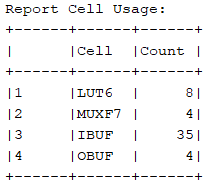
\includegraphics[width=5cm]{{Images/Lut 2.png}}
    \centering
    \caption{This is the LUT list of step 3}
\end{figure}

\begin{figure}[h]
    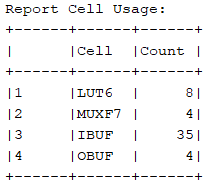
\includegraphics[width=5cm]{{Images/Lut 2.png}}
    \centering
    \caption{This is the LUT list of step 4}
\end{figure}

\begin{figure}[h]
    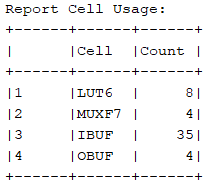
\includegraphics[width=5cm]{{Images/Lut 2.png}}
    \centering
    \caption{This is the LUT list of step 5}
\end{figure}
              
\clearpage

\section{Simulations}


\begin{figure}[h]
    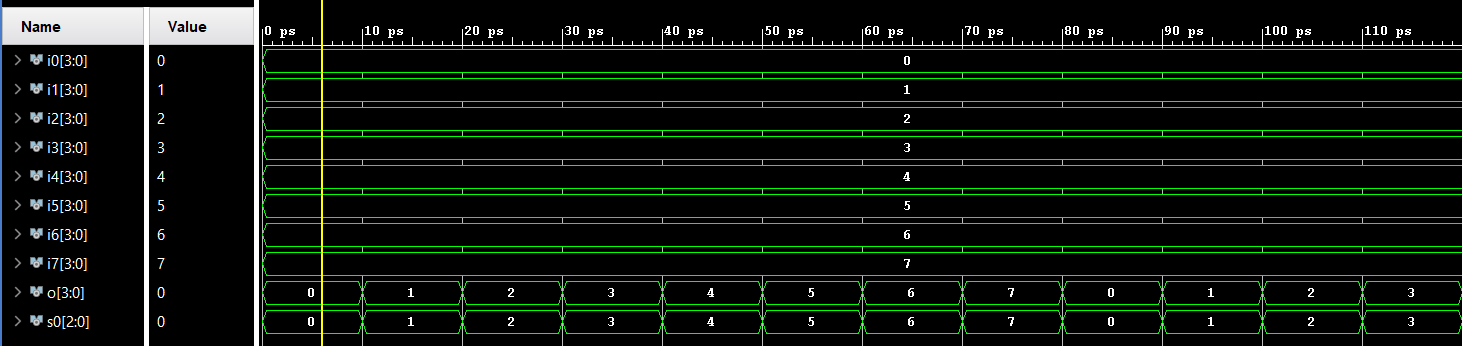
\includegraphics[width=13cm]{{Images/Wave 1.1.png}}
    \centering
    \caption{This is the simulation of step 1}
\end{figure}

\begin{figure}[h]
    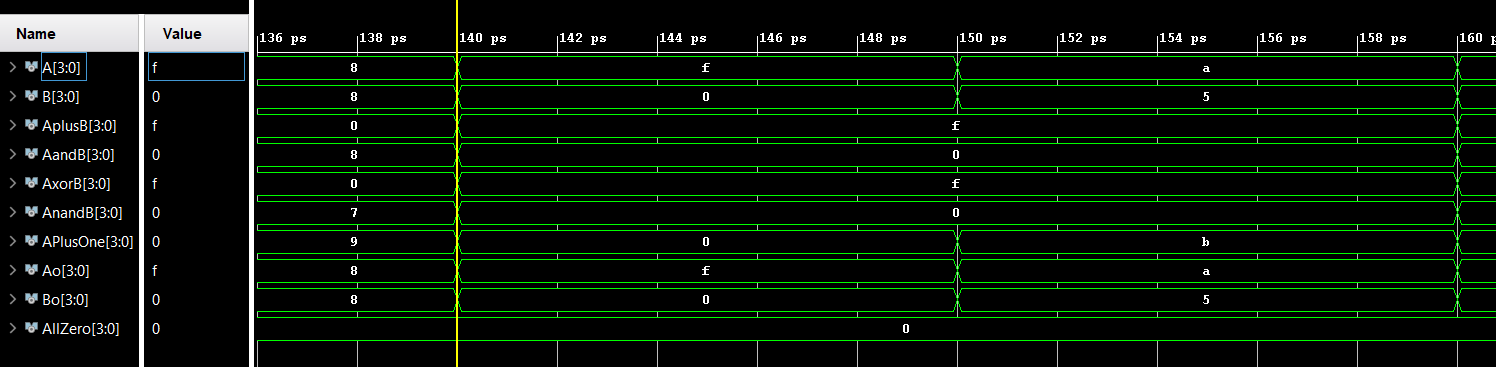
\includegraphics[width=13cm]{{Images/Wave 2.1.png}}
    \centering
    \caption{This is the simulation of step 2}
\end{figure}

\begin{figure}[h]
    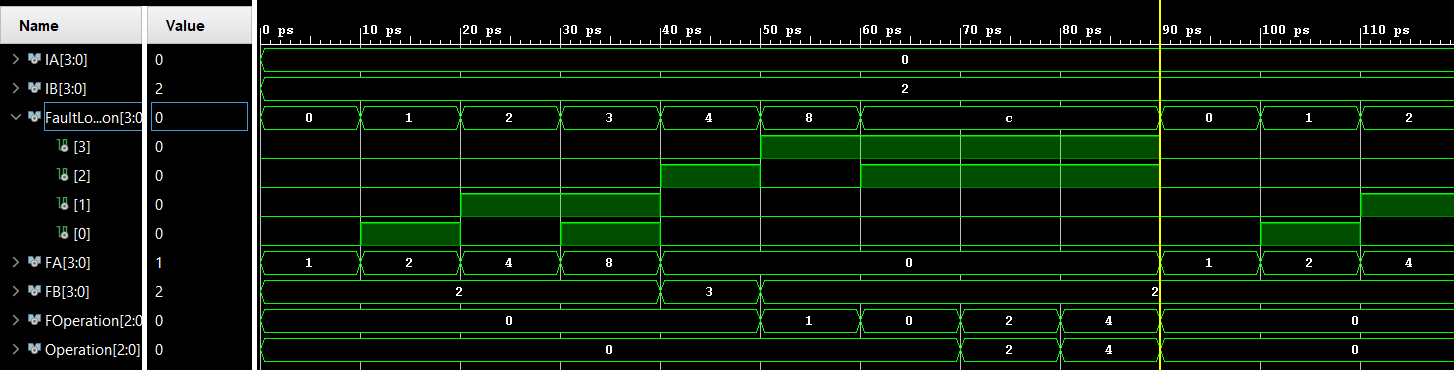
\includegraphics[width=13cm]{{Images/Wave 3.1.png}}
    \centering
    \caption{This is the simulation of step 3}
\end{figure}

\begin{figure}[h]
    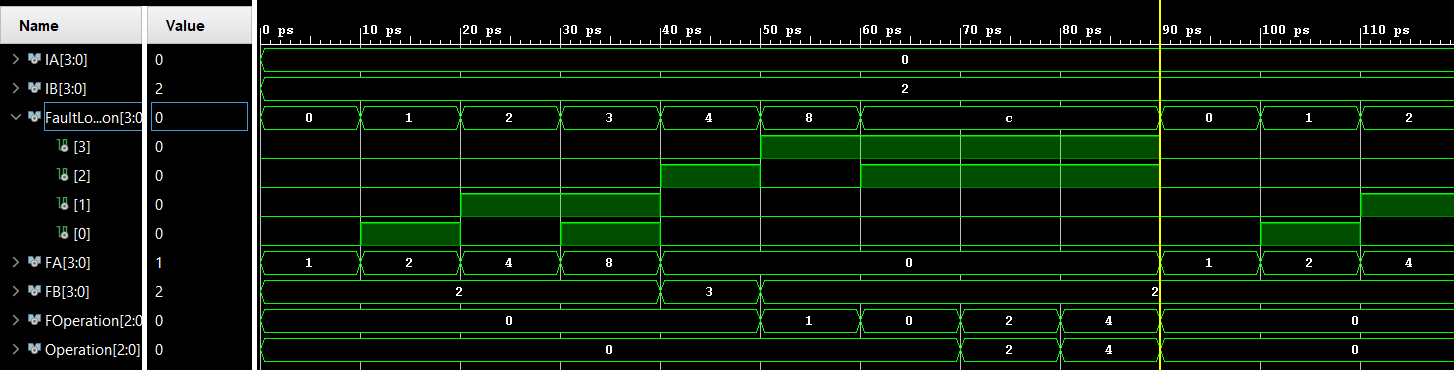
\includegraphics[width=13cm]{{Images/Wave 3.1.png}}
    \centering
    \caption{This is the simulation of step 4}
\end{figure}

\begin{figure}[h]
    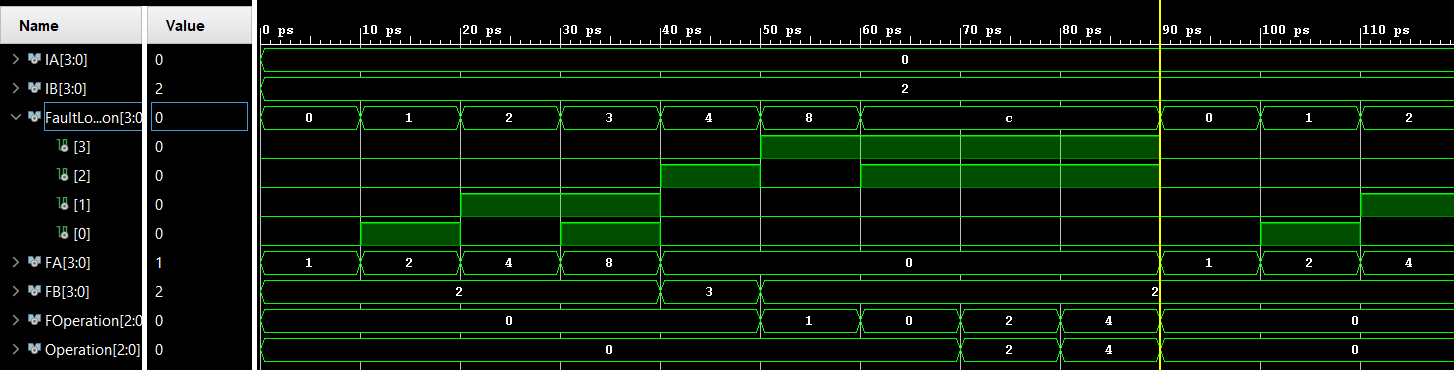
\includegraphics[width=13cm]{{Images/Wave 3.1.png}}
    \centering
    \caption{This is the simulation of step 5}
\end{figure}
\end{document}
